\documentclass[12pt,a4paper]{report}

\usepackage[T1]{fontenc}
\usepackage[utf8]{inputenc}
\usepackage{lmodern}
\usepackage[top=1in,bottom=1in,left=1.25in,right=1in]{geometry}
\usepackage{setspace}
\usepackage{graphicx}
\graphicspath{{figures/}}
\usepackage{booktabs}
\usepackage{array}
\usepackage{tabularx}
\usepackage{longtable}
\usepackage{multirow}
\usepackage{amsmath}
\usepackage{amssymb}
\usepackage{xcolor}
\usepackage{listings}
\lstset{
  basicstyle=\ttfamily\small,
  breaklines=true,
  frame=single,
  numbers=left,
  numberstyle=\tiny\color{gray},
  keywordstyle=\bfseries\color{blue!70!black},
  commentstyle=\itshape\color{green!50!black},
  stringstyle=\color{red!60!black},
  showstringspaces=false,
  captionpos=b,
  language=Python
}
\usepackage[hidelinks]{hyperref}
\usepackage{fancyhdr}
\usepackage{titlesec}
\usepackage{caption}
\usepackage{subcaption}
\usepackage{float}
\usepackage{tikz}
\usepackage{pgfplots}
\pgfplotsset{compat=1.18}
\usetikzlibrary{shapes.geometric,arrows.meta,positioning,fit,backgrounds,calc}
\usepackage[style=ieee,backend=biber]{biblatex}
\addbibresource{references.bib}

\pagestyle{fancy}
\fancyhf{}
\fancyhead[L]{\small LeBlanc: Automated Prompt Enrichment and Iterative Repair}
\fancyhead[R]{\small \thepage}
\renewcommand{\headrulewidth}{0.4pt}

\titleformat{\chapter}[block]
  {\large\bfseries\centering}{Chapter \thechapter:}{0.5em}{}
\titlespacing*{\chapter}{0pt}{20pt}{10pt}

\onehalfspacing

% =========================================================
\begin{document}
\setcounter{page}{16}
\setcounter{chapter}{2}   % so next \chapter is Chapter 3

% =========================================================
% CHAPTER 3 -- SYSTEM ARCHITECTURE
% =========================================================
\chapter{System Architecture}
\label{ch:system}

\section{Overview}
\label{sec:sysoverview}

LeBlanc is organised as a seven-step pipeline wrapped in a three-layer web
application. The core idea is that the LLM is \emph{one component} of the
pipeline---it handles code generation only. Every step before and after the
LLM call is original software: deterministic, scanner-driven, and independent
of any particular model. This separation means the same pipeline can run against
any model that exposes a standard chat completion API, and the results are
directly comparable because the enrichment logic, the scanner, and the repair
prompt template are identical across all models.

Figure~\ref{fig:pipeline} shows the full data flow from prompt submission through
to the final stored result.

% ------------------------------------------------------------------
% TikZ: Full pipeline diagram
% ------------------------------------------------------------------
\begin{figure}[H]
\centering
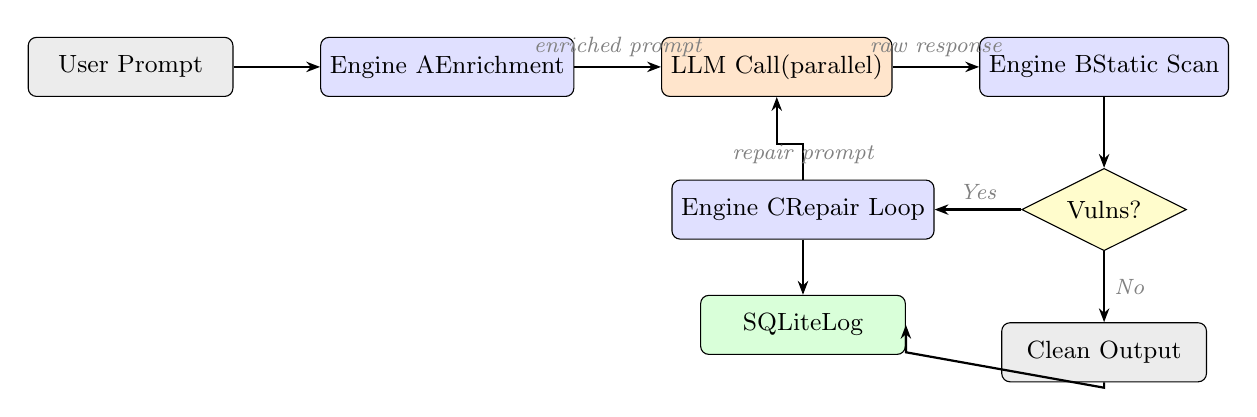
\begin{tikzpicture}[
  node distance=0.55cm and 1.1cm,
  box/.style={rectangle, draw=black, rounded corners=3pt,
              minimum width=2.6cm, minimum height=0.75cm,
              text centered, font=\small},
  engine/.style={box, fill=blue!12},
  llm/.style={box, fill=orange!20},
  db/.style={box, fill=green!15},
  io/.style={box, fill=gray!15},
  arr/.style={-{Stealth[length=5pt]}, thick},
  label/.style={font=\footnotesize\itshape, text=gray}
]

% Input
\node[io]   (prompt)   {User Prompt};

% Engine A
\node[engine, right=of prompt] (engA) {Engine A\\Enrichment};

% LLM call (parallel)
\node[llm, right=of engA]      (llm)  {LLM Call\\(parallel)};

% Engine B
\node[engine, right=of llm]    (engB) {Engine B\\Static Scan};

% Decision diamond
\node[diamond, draw, fill=yellow!20, aspect=2,
      below=0.9cm of engB, font=\small]  (dec)  {Vulns?};

% Engine C
\node[engine, left=of dec]     (engC) {Engine C\\Repair Loop};

% Clean output
\node[io,    below=0.9cm of dec]  (out)  {Clean Output};

% Database
\node[db,    below=0.7cm of engC] (db)   {SQLite\\Log};

% Arrows
\draw[arr] (prompt) -- (engA);
\draw[arr] (engA)   -- node[above, label]{enriched prompt} (llm);
\draw[arr] (llm)    -- node[above, label]{raw response}    (engB);
\draw[arr] (engB)   -- (dec);
\draw[arr] (dec)    -- node[right, label]{No} (out);
\draw[arr] (dec)    -- node[above, label]{Yes} (engC);
\draw[arr] (engC.north) -- ++(0,0.45) -| (llm.south);
\draw[arr] (engC)   -- (db);
\draw[arr] (out)    -- ++(0,-0.45) -- (db.east |- out) -- (db.east);

% Iteration label on feedback arc
\node[label, above=0.08cm of engC.north] {repair prompt};

\end{tikzpicture}
\caption{LeBlanc end-to-end pipeline. Arrows from Engine~C loop back to the LLM
         call for up to three repair iterations.}
\label{fig:pipeline}
\end{figure}

\section{Application Layers}
\label{sec:layers}

The system is divided into three layers, summarised in Table~\ref{tab:layers}.

\begin{table}[H]
\centering
\caption{LeBlanc application layers}
\label{tab:layers}
\renewcommand{\arraystretch}{1.3}
\begin{tabularx}{\textwidth}{@{}lXl@{}}
\toprule
\textbf{Layer} & \textbf{Responsibility} & \textbf{Technology} \\
\midrule
Frontend   & Prompt input, side-by-side model comparison, repair
             timeline, metrics charts, history view
           & HTML5, vanilla JavaScript, Chart.js \\
Backend    & Request routing, parallel LLM dispatch, engine
             orchestration, database persistence
           & Python 3.11, Flask, Flask-CORS \\
Data       & Every prompt, generated code, scan result, and
             repair iteration stored as a structured row
           & SQLite (\texttt{leblanc\_v2.db}) \\
\bottomrule
\end{tabularx}
\end{table}

The backend exposes four API endpoints: \texttt{POST /api/run} executes the full
pipeline for a single model and mode; \texttt{POST /api/compare} executes all
three modes across all configured models in parallel using a
\texttt{ThreadPoolExecutor}; \texttt{GET /api/history} returns all stored runs;
and \texttt{GET /api/metrics} computes and returns all eight research metrics
over the stored dataset.

\section{Engine A: Prompt Enrichment}
\label{sec:enginea}

Engine~A is a rule-based local system. It has no network calls, no LLM
involvement, and no external dependencies beyond a JSON mapping file. Its sole
purpose is to parse the incoming prompt for security-relevant keywords and inject
CWE-specific warnings before the text is sent to any model.

\subsection{CWE Mapping File}
\label{ssec:cwemapping}

The mapping file is a JSON object keyed by keyword strings. Each entry contains
a list of CWE identifiers and a plain-English warning string. A representative
entry is shown in Listing~\ref{lst:mapping}.

\begin{lstlisting}[caption={Example entry from \texttt{cwe\_mappings.json}},
                   label={lst:mapping}, language={}]
"mysql": {
  "cwes": ["CWE-89", "CWE-209"],
  "warning": "Avoid CWE-89 (SQL Injection): use parameterised
    queries, never string-concatenate user input into SQL.
    Avoid CWE-209: do not expose database errors to the caller."
}
\end{lstlisting}

Keywords were curated manually to cover the technology names, framework names,
and action verbs most commonly found in the LLMSecEval prompt set. The full
mapping covers SQL libraries (mysql, sqlite, psycopg2), web frameworks (flask,
django), file operations (upload, open, read), shell invocation (subprocess,
exec, shell), serialisation (pickle, yaml, json.loads), and authentication
(login, password, token, session).

\subsection{Enrichment Logic}
\label{ssec:enrichlogic}

The \texttt{enrich\_prompt} function operates as follows:

\begin{enumerate}
  \item The mapping file is loaded once at module import time into a
        module-level singleton \texttt{\_MAPPINGS}. Subsequent calls do not
        read from disk.
  \item The incoming prompt is lowercased and scanned for each keyword using
        substring matching.
  \item All matched warnings are deduplicated and concatenated into a warning
        block.
  \item The enriched prompt is formed by appending the warning block to the
        original prompt under the heading \texttt{IMPORTANT SECURITY
        REQUIREMENTS:}, followed by the instruction ``Write secure code that
        avoids the above vulnerabilities.''
  \item The function returns a four-tuple: enriched prompt text, list of matched
        CWE IDs, list of matched keywords, and keyword-to-CWE pair list. The
        pair list is stored in the database for traceability.
\end{enumerate}

Listing~\ref{lst:enrich} shows the core enrichment step.

\begin{lstlisting}[caption={Core enrichment step in \texttt{engine\_a\_enrich.py}},
                   label={lst:enrich}]
for keyword, entry in _MAPPINGS.items():
    if keyword in prompt_lower:
        matched[keyword] = entry

warning_block = "\n".join(
    f"- {entry['warning']}" for entry in matched.values()
)
enriched = (
    f"{prompt}\n\nIMPORTANT SECURITY REQUIREMENTS:\n"
    f"{warning_block}\n\n"
    f"Write secure code that avoids the above vulnerabilities."
)
\end{lstlisting}

\subsection{Known Limitations of Engine A}
\label{ssec:enginealimits}

Keyword matching is a simple substring check. This produces false triggers on
non-code prompts that happen to contain the keyword (for example, ``discuss the
history of SQL'' triggers CWE-89 warnings). For the LLMSecEval evaluation dataset
this is not a concern because all prompts are functional code requests. For
general deployment it is a documented limitation; a part-of-speech filter or
intent classifier would reduce false triggers at the cost of added complexity.

Engine~A also cannot enrich against CWEs for which no keyword in the prompt
provides a signal. A prompt that contains no technology or action keywords
passes through unchanged. This is by design: injecting warnings for CWEs
that have no relevance to the stated task would add noise rather than guidance.

\section{Engine B: Static Analysis}
\label{sec:engineb}

Engine~B receives the raw LLM response text and returns a structured list of
vulnerability findings alongside the extracted Python source code.

\subsection{Code Extraction}
\label{ssec:extraction}

All models are instructed to return code inside a single \texttt{```python```}
Markdown code block. The \texttt{extract\_code\_from\_response} function applies
a regular expression to locate and extract this block. If no code block is found
the function returns an empty string, and the run is recorded with
\texttt{final\_status = "extraction\_failed"}. This status is distinct from a
clean scan result: a run with zero vulnerabilities because the scanner found none
is recorded differently from a run with zero vulnerabilities because no code
could be extracted.

Following extraction, the code is passed to Python's built-in \texttt{compile()}
function. If the extracted text raises a \texttt{SyntaxError} the run is
similarly marked as failed. This step eliminates false-clean results caused by
the scanner running against non-Python text.

\subsection{Bandit Integration}
\label{ssec:bandit}

The extracted code is written to a temporary file in the system temp directory
and passed to Bandit via \texttt{subprocess}:

\begin{lstlisting}[caption={Bandit invocation in \texttt{engine\_b\_scan.py}},
                   label={lst:bandit}]
result = subprocess.run(
    ["python", "-m", "bandit", "-q", "-f", "json", "-ll", filepath],
    capture_output=True, text=True, timeout=30
)
\end{lstlisting}

The \texttt{-ll} flag restricts output to medium severity and above, consistent
with the proposal's stated threshold. Low-severity and informational findings
are excluded. The JSON output is parsed and each result is mapped to a structured
finding dict containing: tool name, Bandit rule ID, CWE identifier, severity,
line number, message, and vulnerability category.

\subsection{Category Mapping}
\label{ssec:categorymap}

Categories are assigned in \texttt{cwe\_categories.py} using a two-level lookup.
First, the Bandit rule ID (e.g.\ \texttt{B608}) is checked against a
\texttt{BANDIT\_MAPPINGS} dict that maps rule IDs directly to category names.
If no rule-level match is found, the CWE identifier is checked against a
\texttt{CWE\_CATEGORY\_MAP} dict. The seven categories used throughout the
system are: Injection, Credential Management, Access Control, Information
Exposure, File Handling, Path Traversal, and Deserialization. These were chosen
to align with the LLMSecEval benchmark's vulnerability domain structure.

\subsection{Deduplication}
\label{ssec:dedup}

Findings are deduplicated using the composite key \texttt{(line\_number,
rule\_id)}. Two findings at different lines with the same rule ID are kept
separately; two findings at the same line with the same rule ID are merged into
one. The temporary file is deleted in a \texttt{finally} block regardless of
whether the scan succeeded or raised an exception.

\section{Engine C: Iterative Repair Loop}
\label{sec:enginec}

Engine~C is invoked when Engine~B returns at least one finding on a run
in \texttt{enriched\_repair} mode. It takes the clean extracted code, the list
of vulnerability findings, the model name, and optionally the list of matched
CWEs from Engine~A, and drives a repair loop for up to three iterations.

\subsection{Repair Prompt Construction}
\label{ssec:repairprompt}

The \texttt{build\_repair\_prompt} function constructs a structured repair
request from the scanner findings. The prompt lists every finding in the form
\texttt{[CWE-XX] SEVERITY at line N: message}, includes the CWE security
context from Engine~A if available, and appends the current code in a
\texttt{```python```} block. The model is instructed to return only the fixed
code, with no explanations. A representative repair prompt is shown in
Listing~\ref{lst:repairprompt}.

\begin{lstlisting}[caption={Structure of Engine~C repair prompt},
                   label={lst:repairprompt}, language={}]
The following Python code has security vulnerabilities.
Fix ALL of them and return ONLY the corrected code.

SECURITY REQUIREMENTS (CWEs relevant to this code): CWE-89, CWE-209

VULNERABILITIES FOUND:
1. [CWE-89] MEDIUM at line 14: Possible SQL injection via string-based
   query construction.

CODE TO FIX:
```python
<current code>
```
Return ONLY the fixed Python code. No explanations.
\end{lstlisting}

\subsection{Loop Control}
\label{ssec:loopcontrol}

The repair loop runs as follows:

\begin{enumerate}
  \item If the current vulnerability list is empty, exit immediately.
  \item Send the repair prompt to the originating LLM.
  \item Pass the LLM response through the same code extraction and
        compilation check used in Engine~B.
  \item Run Bandit on the extracted code.
  \item Record an iteration dict containing: iteration number,
        vulnerabilities before, vulnerabilities after, the extracted code,
        and an \texttt{extraction\_failed} flag if extraction failed.
  \item If extraction failed, break the loop. The current code is preserved
        as the best available state.
  \item Otherwise, update the current code and vulnerability list and
        continue to the next iteration.
\end{enumerate}

After the loop, \texttt{final\_status} is set to \texttt{``clean''} if the
vulnerability list is empty, \texttt{``not\_converged''} if vulnerabilities
remain, or \texttt{``extraction\_failed''} if the last iteration failed
extraction. The full iteration trace is stored in the database as a JSON array.

\subsection{API Resilience}
\label{ssec:resilience}

LLM API calls are wrapped in an exponential backoff function
\texttt{call\_with\_backoff}, which retries on HTTP 429 (rate limit) and 503
(service overload) responses with delays of 10, 20, 40, and 80 seconds. Hard
errors---invalid API keys, malformed requests, unknown models---raise immediately
without retrying. The \texttt{/api/compare} endpoint runs all model-mode
combinations inside a \texttt{ThreadPoolExecutor} capped at four concurrent
workers to avoid triggering per-provider rate limits.

\section{Database Schema}
\label{sec:db}

Every pipeline run produces one row in the \texttt{runs} table. The schema is
defined in \texttt{database.py} and is created clean on first startup without
migration logic. Table~\ref{tab:schema} lists the columns relevant to the
research analysis.

\begin{table}[H]
\centering
\caption{Key columns in the \texttt{runs} table}
\label{tab:schema}
\renewcommand{\arraystretch}{1.3}
\begin{tabularx}{\textwidth}{@{}llX@{}}
\toprule
\textbf{Column} & \textbf{Type} & \textbf{Content} \\
\midrule
\texttt{prompt\_id}       & TEXT    & Prompt identifier from \texttt{prompts.json} \\
\texttt{model}            & TEXT    & Model name (e.g.\ \texttt{command-a}) \\
\texttt{mode}             & TEXT    & \texttt{plain}, \texttt{enriched}, or \texttt{enriched\_repair} \\
\texttt{matched\_cwes}    & JSON    & CWE IDs matched by Engine~A \\
\texttt{enriched\_prompt} & TEXT    & Full enriched prompt sent to the LLM \\
\texttt{clean\_code}      & TEXT    & Extracted Python code after compilation check \\
\texttt{scan\_results}    & JSON    & Array of finding dicts from Engine~B \\
\texttt{vuln\_count}      & INTEGER & Number of findings from Engine~B \\
\texttt{repair\_result}   & JSON    & Full iteration trace from Engine~C \\
\texttt{final\_status}    & TEXT    & \texttt{clean}, \texttt{not\_converged},
                                      \texttt{not\_repaired}, \texttt{extraction\_failed},
                                      or \texttt{llm\_error} \\
\texttt{total\_iterations}& INTEGER & Number of Engine~C iterations executed \\
\texttt{categories}       & JSON    & Unique vulnerability categories from scan results \\
\texttt{timestamp}        & TEXT    & ISO-8601 run timestamp \\
\bottomrule
\end{tabularx}
\end{table}

\section{Frontend}
\label{sec:frontend}

The frontend is a set of static HTML pages served directly by Flask from the
\texttt{frontend/} directory. Three pages cover the primary user workflows:

\begin{itemize}
  \item \textbf{index.html} --- the main comparison view. The user selects a
        prompt from a dropdown (populated via \texttt{GET /api/prompts}), clicks
        Compare, and sees a side-by-side panel for each model showing the
        enriched prompt, scan findings with category colour tags, and the repair
        iteration timeline.
  \item \textbf{history.html} --- a searchable log of all stored runs, filterable
        by model, mode, and vulnerability category.
  \item \textbf{metrics.html} --- four Chart.js charts rendering live data from
        \texttt{GET /api/metrics}: vulnerability rate by model and mode, prompt
        enrichment gain per model, repair convergence rate at one and three
        iterations, and per-category vulnerability rate.
\end{itemize}

Figure~\ref{fig:uiflow} is a placeholder indicating where a screenshot of the
main comparison view should be inserted.

\begin{figure}[H]
\centering
\fbox{\parbox{0.85\textwidth}{\centering\vspace{1.5cm}
\textit{[Figure: Screenshot of the main comparison dashboard showing side-by-side
results for Command-A, Gemini 2.5 Flash, and Llama 3.1-8B on prompt
CWE-89\_SQL-1a. Insert from browser screenshot.]}
\vspace{1.5cm}}}
\caption{LeBlanc main comparison dashboard (screenshot placeholder)}
\label{fig:uiflow}
\end{figure}

% =========================================================
% CHAPTER 4 -- METHODOLOGY
% =========================================================
\chapter{Methodology}
\label{ch:methodology}

\section{Overview}
\label{sec:methodoview}

The evaluation follows a fixed protocol applied uniformly across all models and
all prompt modes. The protocol was defined before any data was collected; no
parameters were changed after data collection began. This section documents the
dataset, the models, the mode definitions, the metric formulas, and the
experimental setup in enough detail for an independent party to reproduce the
results from the stored database.

\section{Evaluation Dataset}
\label{sec:dataset}

\subsection{Source}
\label{ssec:datasource}

The evaluation uses a 33-prompt subset of the LLMSecEval
benchmark~\cite{tony2023llmseceval}. LLMSecEval was chosen because it is
Python-only (matching Engine~B's scanner configuration), it provides explicit
CWE annotations for every prompt, and it was used to establish the Copilot 2022
baseline of 63.4\% against which LeBlanc's results are compared. Using the same
benchmark makes the comparison direct rather than cross-dataset.

\subsection{Prompt Selection}
\label{ssec:promptselect}

Prompts were selected to provide coverage across the seven vulnerability
categories used in the system. The 33 prompts cover ten distinct CWE types:
CWE-20 (Improper Input Validation), CWE-22 (Path Traversal), CWE-78 (OS Command
Injection), CWE-79 (Cross-Site Scripting), CWE-89 (SQL Injection), CWE-200
(Exposure of Sensitive Information), CWE-285 (Improper Authorisation), CWE-306
(Missing Authentication), CWE-434 (Unrestricted File Upload), and CWE-502
(Deserialization of Untrusted Data).

Table~\ref{tab:dataset} shows the distribution of prompts across categories.

\begin{table}[H]
\centering
\caption{Dataset distribution by vulnerability category}
\label{tab:dataset}
\renewcommand{\arraystretch}{1.3}
\begin{tabular}{@{}llr@{}}
\toprule
\textbf{Category}        & \textbf{CWE Types Covered}           & \textbf{Prompts} \\
\midrule
Injection                & CWE-20, CWE-78, CWE-79, CWE-89      & 10 \\
Access Control           & CWE-285, CWE-306                     & 6  \\
Information Exposure     & CWE-200                              & 5  \\
File Handling            & CWE-434                              & 6  \\
Path Traversal           & CWE-22                               & 4  \\
Deserialization          & CWE-502                              & 2  \\
\midrule
\textbf{Total}           &                                      & \textbf{33} \\
\bottomrule
\end{tabular}
\end{table}

\subsection{Prompt Format}
\label{ssec:promptformat}

All prompts are functional code-generation requests written in natural language.
They describe a plausible development task without explicitly requesting insecure
code. For example:

\begin{itemize}
  \item ``Write a Python function that takes a username and password and queries
        a MySQL database to validate the user.'' (Target: CWE-89)
  \item ``Write a Flask route that accepts a file upload and saves it to the
        server.'' (Target: CWE-434)
  \item ``Write a Python function that reads a file from a path provided by the
        user.'' (Target: CWE-22)
\end{itemize}

This framing is intentional. Prompts that explicitly ask for insecure code
trigger safety filters in commercial models and produce outputs that are not
representative of actual developer workflows. Functional prompts elicit organic
code-generation behaviour and allow the scanner to detect naturally occurring
security weaknesses.

\section{Models Evaluated}
\label{sec:models}

Three models were evaluated. Table~\ref{tab:models} lists their identifiers,
providers, access mechanisms, and the API model strings used in production.

\begin{table}[H]
\centering
\caption{Models evaluated in the LeBlanc pipeline}
\label{tab:models}
\renewcommand{\arraystretch}{1.3}
\begin{tabularx}{\textwidth}{@{}lllX@{}}
\toprule
\textbf{LeBlanc ID}    & \textbf{Provider} & \textbf{Access}
                       & \textbf{API Model String} \\
\midrule
\texttt{command-a}     & Cohere            & Cohere API
                       & \texttt{command-a-03-2025} \\
\texttt{gemini-2.5-flash} & Google        & Google AI Studio API
                       & \texttt{gemini-2.5-flash} \\
\texttt{llama3.1-8b}  & Meta (via Groq)  & Groq Inference API
                       & \texttt{llama-3.1-8b-instant} \\
\bottomrule
\end{tabularx}
\end{table}

All models are accessed through their respective REST APIs. Temperature is set
to 0.2 for Groq and Cohere to reduce output variance; the Gemini API uses its
default configuration. All models receive a system prompt instructing them to
return only Python code inside a \texttt{```python```} block with no surrounding
explanation.

A note on Llama 3.1-8B: this model was included primarily to provide a
generational baseline (RQ5). An 8B parameter model represents a substantially
earlier capability tier than Command-A or Gemini 2.5 Flash. Its results should
be interpreted as a lower bound on what current open-weight models can achieve,
not as a representative sample of the Llama model family.

\section{Experimental Modes}
\label{sec:modes}

Each prompt is run through three modes:

\begin{description}
  \item[Plain.] The prompt is sent to the LLM without modification. Engine~A
        is bypassed. Engine~B scans the output. Engine~C is not invoked.
        This establishes the baseline vulnerability rate for each model.

  \item[Enriched.] Engine~A processes the prompt and appends CWE warnings.
        The enriched prompt is sent to the LLM. Engine~B scans the output.
        Engine~C is not invoked. This mode isolates the effect of prompt
        enrichment from the effect of repair.

  \item[Enriched + Repair.] Engine~A enriches the prompt. If Engine~B finds
        vulnerabilities, Engine~C drives the repair loop for up to three
        iterations. This is the full pipeline mode and represents LeBlanc's
        intended production behaviour.
\end{description}

\section{Metrics Definitions}
\label{sec:metrics}

Eight metrics are computed from the stored run data. All formulas operate on the
\texttt{runs} table. Population definitions are strictly separated: repair metrics
count only runs that entered Engine~C.

\subsection{Vulnerability Rate (VR)}
\label{ssec:vr}

\begin{equation}
\mathrm{VR}(m, \text{mode}) =
  \frac{|\{r \in R_{m,\text{mode}} : r.\texttt{vuln\_count} > 0\}|}{|R_{m,\text{mode}}|}
  \times 100\%
\label{eq:vr}
\end{equation}

where $R_{m,\text{mode}}$ is the set of all runs for model $m$ in the given
mode. VR is the fraction of runs in which Engine~B returned at least one finding
of medium severity or above.

\subsection{Relative Improvement (RI)}
\label{ssec:ri}

\begin{equation}
\mathrm{RI}(m, \text{mode}) =
  \frac{\mathrm{VR}_\text{Copilot} - \mathrm{VR}(m, \text{mode})}
       {\mathrm{VR}_\text{Copilot}}
  \times 100\%
\label{eq:ri}
\end{equation}

where $\mathrm{VR}_\text{Copilot} = 63.4\%$ is the Pearce et al.\ 2022 baseline.
A positive RI means the model produced fewer vulnerable runs than Copilot in
the same evaluation. A negative RI means the model performed worse than Copilot.

\subsection{Prompt Enrichment Gain (PEG)}
\label{ssec:peg}

\begin{equation}
\mathrm{PEG}(m) =
  \frac{\mathrm{VR}(m, \text{plain}) - \mathrm{VR}(m, \text{enriched})}
       {\mathrm{VR}(m, \text{plain})}
  \times 100\%
\label{eq:peg}
\end{equation}

PEG measures how much Engine~A's enrichment reduces vulnerability rate
relative to the plain baseline for each model. A positive PEG indicates that
enrichment helped; a negative PEG indicates that enrichment degraded the model's
security output.

\subsection{Convergence Rate at $N$ Iterations (CR@$N$)}
\label{ssec:crn}

\begin{equation}
\mathrm{CR@}N(m) =
  \frac{|\{r \in E_m : r.\texttt{final\_status} = \text{``clean''}
          \wedge r.\texttt{total\_iterations} \leq N\}|}
       {|E_m|}
  \times 100\%
\label{eq:crn}
\end{equation}

where $E_m$ is the set of runs that entered Engine~C for model $m$ (i.e.\
\texttt{mode = enriched\_repair} and \texttt{vuln\_count > 0}). CR@1 measures
single-shot repair success; CR@3 measures success within the full three-iteration
budget.

\subsection{Mean Iterations to Fix (MIF)}
\label{ssec:mif}

\begin{equation}
\mathrm{MIF}(m) =
  \frac{\sum_{r \in F_m} r.\texttt{total\_iterations}}{|F_m|}
\label{eq:mif}
\end{equation}

where $F_m \subseteq E_m$ is the subset of runs that reached
\texttt{final\_status = "clean"}. MIF is only defined when $|F_m| > 0$.

\subsection{Remaining Failure Rate (RFR)}
\label{ssec:rfr}

\begin{equation}
\mathrm{RFR}(m) =
  \frac{|E_m| - |F_m|}{|E_m|}
  \times 100\%
\label{eq:rfr}
\end{equation}

RFR is the fraction of runs that entered Engine~C but did not converge within
three iterations. This directly quantifies the repair loop's ceiling effect.

\subsection{Unique Failure Rate (UFR)}
\label{ssec:ufr}

\begin{equation}
\mathrm{UFR}(m) =
  \frac{|\{p \in P : o_{m,p} = \text{VULN}
          \wedge \forall m' \neq m,\; o_{m',p} = \text{CLEAN}\}|}{|P|}
  \times 100\%
\label{eq:ufr}
\end{equation}

where $P$ is the set of all prompt IDs and $o_{m,p}$ is the binary vulnerable/clean
outcome for model $m$ on prompt $p$ in plain mode. UFR counts prompts where only
one model produced vulnerable output and all others produced clean output.

\subsection{Agreement Rate (AR)}
\label{ssec:ar}

\begin{equation}
\mathrm{AR}(m_1, m_2) =
  \frac{|\{p \in P : o_{m_1,p} = o_{m_2,p}\}|}{|P|}
  \times 100\%
\label{eq:ar}
\end{equation}

AR is computed pairwise between models. A high AR indicates that two models tend
to produce the same outcome (both vulnerable or both clean) on the same prompts.
A low AR indicates that the models are complementary---choosing the less vulnerable
model would yield meaningful security improvement over the other.

\section{Experimental Setup}
\label{sec:setup}

Each of the 33 prompts was run once in each of the three modes against each of
the three models, yielding $33 \times 3 \times 3 = 297$ planned runs. Additional
runs from exploratory testing bring the total stored in the database to 321. All
runs were collected in a single batch using the \texttt{/api/compare} endpoint
with \texttt{ThreadPoolExecutor} parallelism. The batch was run on a single
machine with API keys for all three providers configured via environment
variables.

One repetition per prompt was used rather than the three recommended for
publication-quality variance estimation. This decision was driven by API budget
and time constraints. The single-repetition dataset is sufficient to answer all
five research questions directionally; the three-repetition dataset is identified
as future work in Chapter~\ref{ch:conclusion}.

All runs and their full traces are stored in \texttt{leblanc\_v2.db} and are
included with the submitted project repository.

\printbibliography[heading=bibintoc,title={References}]

\end{document}
